\section{Implementación}
En la siguiente sección se presentan los componentes elegidos y sus funciones en el
sistema.
\subsection{Configuración del Pipeline}
\begin{itemize}
	\item \textbf{WhitespaceTokenizer}: componente que divide el texto en palabras
	      individuales, utilizando espacios en blanco como delimitador.
	      \cite{Configuration_Documentation}
	\item \textbf{RegexFeaturizer}: componente que crea características basadas en expresiones
	      regulares. Esto puede ser útil para detectar patrones en el texto.
	      \cite{Configuration_Documentation}
	\item \textbf{LexicalSyntacticFeaturizer}: componente que combina características léxicas y
	      sintácticas para crear una mejor representación del texto. Utiliza etiquetas de
	      partes del discurso
	      y etiquetas de análisis de dependencia para crear características.
	      \cite{Configuration_Documentation}
	\item \textbf{CountVectorsFeaturizer}: componente que crea una representación dispersa de
	      bolsa de
	      palabras del texto. Puede ser utilizado para crear características para la
	      clasificación de
	      intenciones o la extracción de entidades. \cite{Configuration_Documentation}
	\item \textbf{DIETClassifier}: componente que combina una red neuronal recurrente con un
	      transformador para realizar la clasificación de intenciones y el reconocimiento de
	      entidades.
	      Utiliza múltiples fuentes de información, como incrustaciones de palabras,
	      incrustaciones de
	      caracteres y etiquetas de partes del discurso. \cite{Configuration_Documentation}
	\item \textbf{EntitySynonymMapper}: componente que mapea las entidades a su forma canónica. Esto puede ser útil para manejar variaciones en la forma en que se expresan las entidades o como se conocen en RASA 'sinónimos'\cite{Configuration_Documentation}
	\item \textbf{ResponseSelector}: componente que selecciona una respuesta basada en la
	      entrada del
	      usuario. Utiliza un enfoque basado en recuperación, donde coincide la entrada del
	      usuario con un
	      conjunto de respuestas predefinidas. Puede ser útil para manejar preguntas frecuentes
	      o
	      conversaciones informales.\cite{Configuration_Documentation}
	\item \textbf{FallbackClassifier}: componente que clasifica los mensajes como fallback si no coinciden con ninguna de las intenciones en el modelo. Puede ser útil para manejar mensajes fuera de contexto o solicitudes que el modelo no está entrenado para manejar.\cite{Configuration_Documentation}
\end{itemize}
\subsection{Docker}

Para implemtar los servicios se usaron microcontenedores Docker, por lo que introduciremos
brevemente los conceptos de esta tecnología.

\subsection{Contenedor}

Los contenedores son la unidad más pequeña un sistema, es una entidad que se utiliza para aislar
cada componente del sistema base. Cada contenedor puede aislarse mediante funciones del sistema
operativo llamadas cgroups y cnames logrando así aplicaciones en entornos aislados (sandbox en
Ingles). \cite{Docker}
\begin{figure}[H]
\begin{centering}
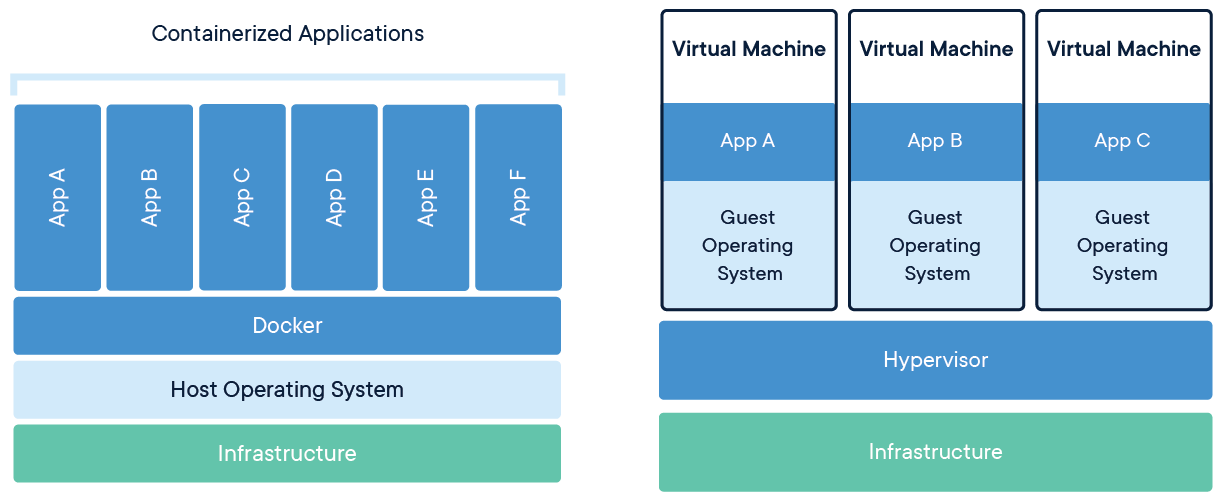
\includegraphics[angle=0,width=0.3\textwidth]{Figuras/docker-container.png}
\par \end{centering}
\caption[Contenedores]{Contenedores. \textbf{Fuente:} \cite{Docker}}
\label{Contenedores}
\end{figure}

\subsection{Imagen de contenedor}
Una imagen de contenedor es el sistema de archivos aislados de todos los archivos necesarios para
ejecutar la aplicación, así como dependencias, configuraciones, ejecutables, etc. Así como también
variables de entorno y datos necesarios para ejecutar la aplicación. \cite{Docker}

\subsection{Redes}
Entre las ventajas de desplegar una aplicación por medio de contenedores Docker es que se pueden
comunicar entre ellos y también con servicios externos al entorno de Docker. Por defecto se pueden
crear varios tipos de configuraciones de red, pero por lo general se utilizan redes puente entre
los contenedores para que estos puedan comunicarse mutuamente entre ellos y solo exponiendo los
puertos necesarios para interactuar con el sistema en cuestión y esta es la opción utilizada en
nuestra implementación. \cite{Docker}

\subsection{Volumenes}
Puesto que un contenedor no tiene un estado persistente sobre los datos que genera, se introducen
los volúmenes, son la forma recomendada de agregar persistencia de datos a un contendedor de Docker. \cite{Docker}
\begin{figure}[H]
\begin{centering}
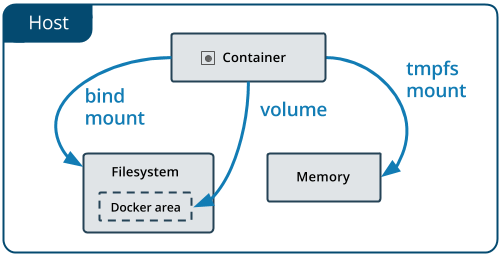
\includegraphics[angle=0,width=0.3\textwidth]{Figuras/docker-volume.png}
\par \end{centering}
\caption[Volumen]{Volumen. \textbf{Fuente:} \cite{Docker}}
\label{Volumen}
\end{figure}

\subsection{Construcción}
Las imágenes de Docker se construyen partir de instrucciones escritas en un archivo denominadado Dockerfile, generalmente de parte de una imagen base de la cual sé la adiciona lo necesario para ejecutar la aplicación.
\cite{Docker}

\subsection{Repositorios}
Un repositorio de imágenes Docker (Docker Registry) es un servidor que almacena y distribuye imágenes versionadas generadas partir de un Dockerfile. Estos repositorios pueden ser públicos como
DockerHub que es el oficial de la comunidad de Docker, como así también privado para un equipo de
desarrollo en una institución. \cite{Docker}

\subsection{Componentes}
Cada componente del sistema se configuró en un contenedor de Docker con la excepción del servidor NGINX que si estaba instalado sobre el sistema operativo del servidor. 
\begin{figure}[H]
\begin{centering}
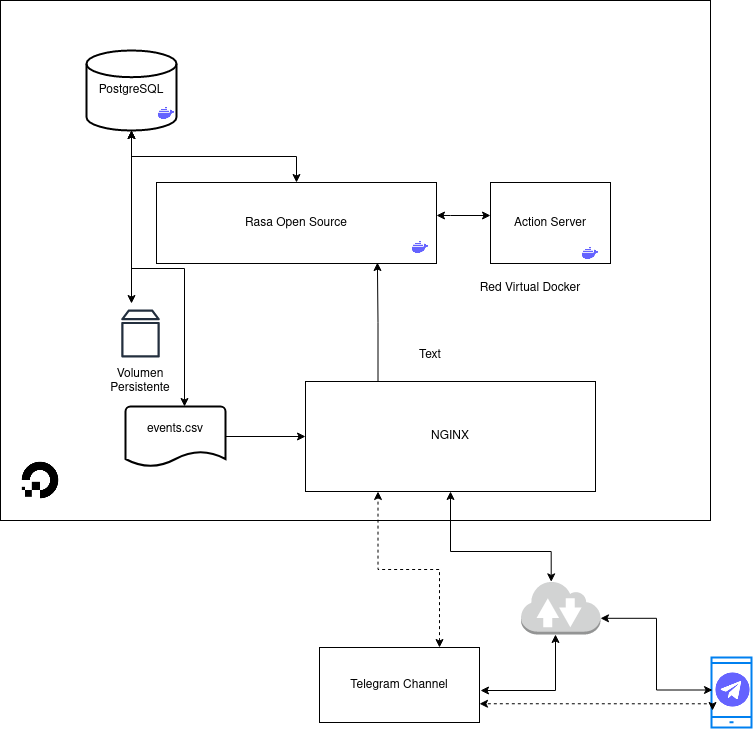
\includegraphics[angle=0,width=0.3\textwidth]{Figuras/server.png}
\par \end{centering}
\caption[Componentes del Sistema]{Componentes del Sistema. \textbf{Fuente:} Elaboración propia.}
\label{Componentes}
\end{figure}
\subsection{Rasa Open Source}
El contendedor de Rasa Open Source ejecuta una imagen oficial proveída por Rasa disponible en los repositorios de DockerHub \cite{DockerHub}, pero con el modelo entrenado y las configuraciones
particulares al proyecto. Es el único contenedor que tiene un puerto externo para servir al usuario. También hace uso de los servicios de PosgresSQL y del servicio de acciones (action server).

\subsection{Servidor de acciones}
Servidor de acciones (acction server) es un servicio interno que ejecuta código escrito en Python este utiliza una imagen oficial para servicios Python disponible en los repositorios de
DockerHub \cite{DockerHub}, estas son operaciones específicas para algunas acciones, una respuesta no estática, como por el ejemplo la acción relacionada con el cálculo de puntajes en el final de acuerdo a los puntajes en los exámenes parciales.

\subsection{PostgresSQL}
PostgresSQL es un motor de base de datos del tipo relacional\cite{postgresql} el cual se configuró
a partir de una imagen oficial de PostgresSQL disponible en los repositorios de DockerHub \cite{DockerHub}. Aparte de sus funciones de base de datos de sistema, también ejecutar un
trabajo periódico (cada una hora) para realizar una copia actualizada de los contenidos de la tabla
Eventos a un archivo separado por comas (csv) que se utiliza para retroalimentar las conversaciones y generar más datos para mejorar el modelo.

\subsection{NGINX}

NGINX, es un servidor web que también puede ser usado como proxy reverso, que implica redirigir el
tráfico a puertos internos y también para servir archivos que fueron las funciones utilizadas para
el proyecto. Así como también puede ser utilizado como balanceador de carga, mail proxy y HTTP
cache, entre otras funciones. \cite{NGINX}\\
El servidor NGINX redirige el tráfico a la instancia de Rasa Open Source y también sirve el archivo de la copia más reciente de la tabla Eventos para agilizar las verificaciones de las respuestas y
preguntas recibidas.

\subsection{Recursos}

Para la puesta en producción del proyecto, se utilizó una instancia de Droplet alojado en Nueva
York del proveedor DigitalOcean con un procesador con un 1vcpu(procesador virtualizado), 1 GB de
RAM, 25 GB de almacenamiento y con un costo de entre 4 y 6 dólares americanos al mes dependiendo
del tráfico presentado. Por las limitaciones de memoria del servidor se configuró también 4 GB de
espacio de intercambio(SWAP) en el espacio de almacenamiento.

\subsection{Telegram}

Para habilitar pruebas para el público general se eligió Telegram, puesto que es bastante sencillo
usar su servicio para conectar a implementaciones de chatbots y este no tiene costo de uso.
\cite{botfather}

\section{Resultados}
Inicialmente, se creó un conjunto de datos con las posibles preguntas frecuentes de los alumnos,
una vez que el Bot estuvo en funcionamiento e integrado a Telegram se recolectaron las preguntas
que realmente tienen los estudiantes de la FIUNA, estas fueron guardadas en una base de datos como
eventos, teniendo mucha información innecesaria para el conjunto de datos. Para un mejor manejo y
limpieza de los datos se utilizó Python con ayuda de la librería Pandas. Posteriormente se guardó
el dataframe creado en un archivo de Excel donde se analizaron y clasificaron un total de 1051
entradas en 141 intenciones distintas, De entre ellas, se identificaron las 15 intenciones más
recurrentes.

\begin{figure}[H]
	\centering
	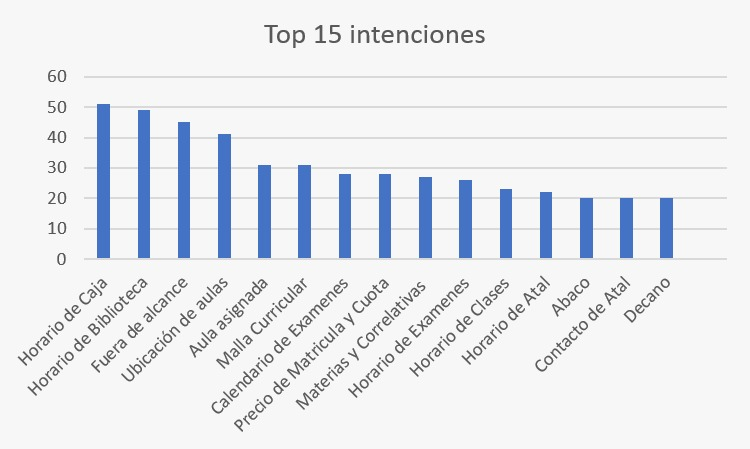
\includegraphics[angle=0,width=0.3\textwidth]{Figuras/Top15intents.jpeg}
	\caption{Top 15 Intenciones}
	\label{fig:Top15intents}
\end{figure}

\subsection{Validación de los datos e Historias}
Rasa cuenta con varias funciones para probar los diálogos, historias, gestor de diálogos y el
procesamiento de mensajes, de tal forma a encontrar errores o inconsistencias antes de realizar el
entrenamiento.

\subsubsection{Validación de datos}
El siguiente comando se encarga de verificar que no haya errores e inconsistencias en los datos y
configuraciones.

\begin{center}
	\framebox[5cm][c]{rasa data validate}
\end{center}

Es recomendable ejecutarlo antes de entrenar el modelo, ya que si se encuentra algún problema, el
entrenamiento también podría fallar.

\subsection{Evaluación del desempeño de la NLU}
Una práctica usual al ejecutar aprendizaje automático es dividir aleatoriamente el conjunto de
datos en uno de entrenamiento y otro de pruebas. El bot utiliza el primer conjunto para aprender
las características necesarias para realizar las predicciones adecuadas, y el segundo conjunto para
evaluar el modelo mediante datos que aún no hayan sido vistos antes.\\
Rasa nos permite dividir los datos mediante el comando:

\begin{center}
	\framebox[5cm][c]{rasa data split nlu}
\end{center}

Por defecto, Rasa separa los datos de entrenamiento/prueba en un 80/20, luego, para probar que tan
bien entrenado se encuentra el modelo utilizamos 'rasa test nlu' especificando cuales son los datos
de entrenamiento y prueba de la siguiente forma:\\

\begin{center}
	\framebox[7cm][c]{    --nlu train\_test\_split/test\_data.yml}
\end{center}

Rasa test proporciona herramientas que facilitan la detección y corrección de errores, incluye una
matriz de confusión, un archivo .json de reporte, un histograma de confianza y un archivo .json de
errores en caso de que existan.\\
\indent La matriz de confusión es una herramienta fundamental que permite evaluar el rendimiento de un
modelo, permite identificar los falsos positivos y falsos negativos, nos muestra en su eje vertical las etiquetas reales y en el eje horizontal las etiquetas predecidas, permitiendo identificar si
existen errores de clasificación.\\
\indent Además, el script de rasa test guarda estos errores de clasificación en un archivo .json lo que
facilita el depurado y corrección de errores para mejorar la calidad de la clasificación.\\
\indent El Histograma nos permite visualizar las predicciones del modelo y la confianza que ha sido
otorgada a cada intención o entidad.\\
\indent Las predicciones correctas se encuentran en la parte izquierda del gráfico y son representadas en
color azul, mientras que las incorrectas se encuentran a la derecha y son de color rojo.\\
\indent La ubicación de cada predicción en el eje horizontal del histograma representa el número de
muestras, y en el eje vertical la confianza con la que el modelo ha realizado su predicción. \cite{interpretacion_graficos}

\subsubsection{Clasificador de Intenciones}
Al analizar la matriz de confusión \ref{fig:intent_matriz} y el histograma
\ref{fig:intent_histograma} podemos verificar que todas las intenciones fueron clasificadas
correctamente con una confianza superior a 0.98, indicando que el modelo es bastante efectivo en su
tarea de clasificación.
\begin{figure}[H]
	\centering
	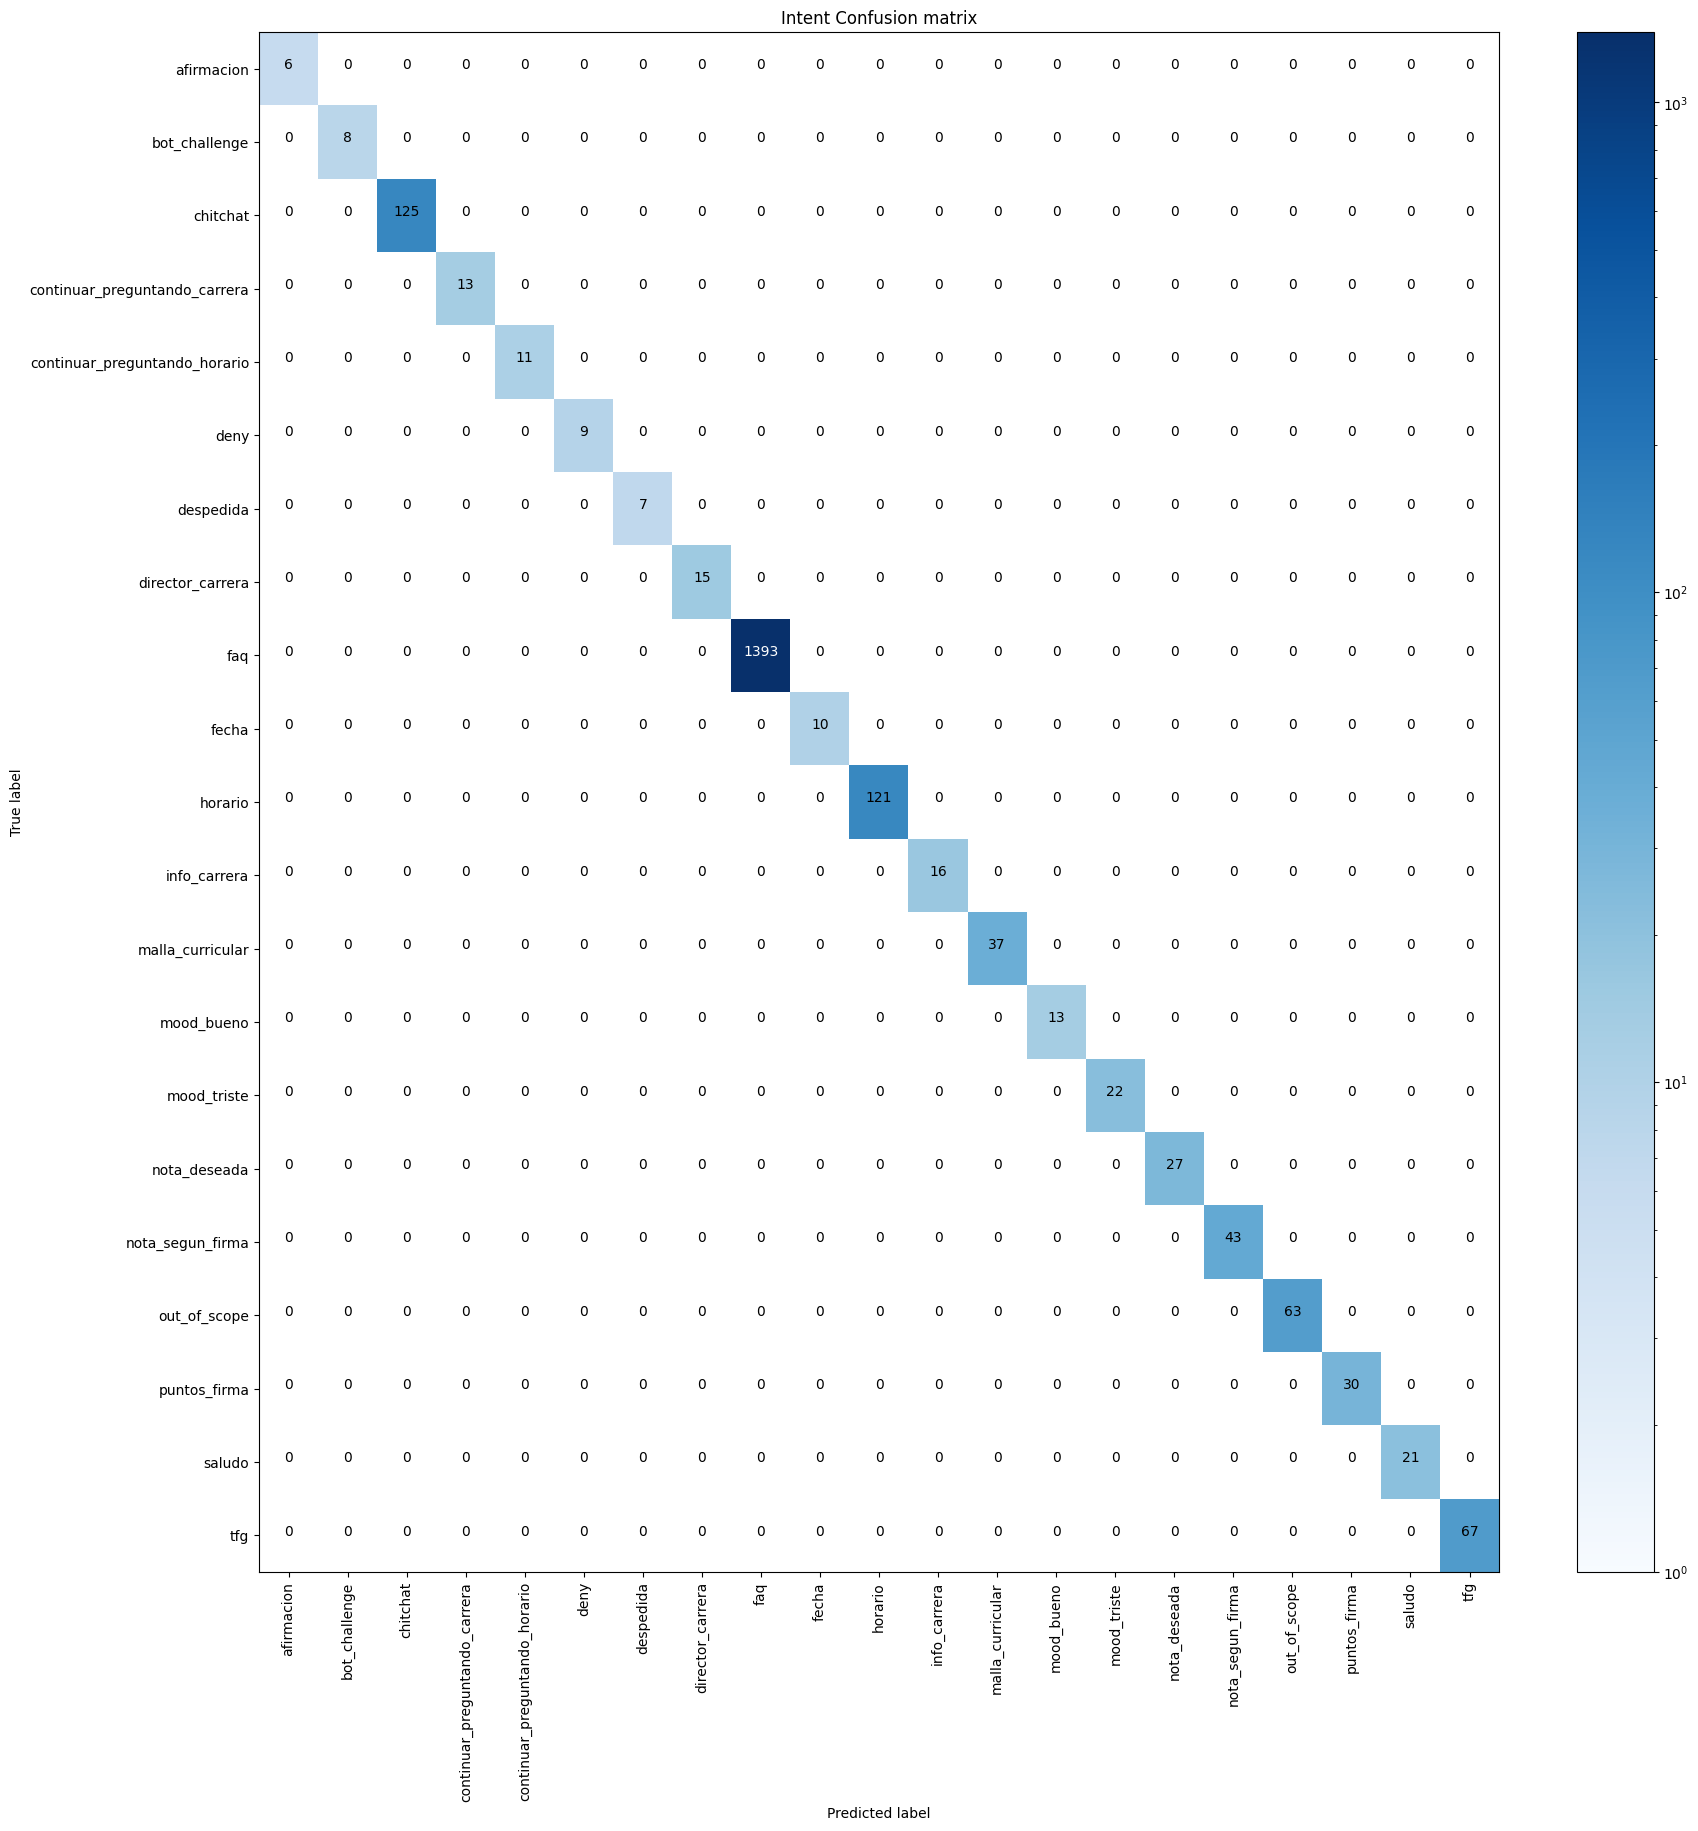
\includegraphics[angle=0,width=0.3\textwidth]{Figuras/intent_confusion_matrix.png}
	\caption{Matriz de Confusión de Intenciones}
	\label{fig:intent_matriz}
\end{figure}

\begin{figure}[H]
	\centering
	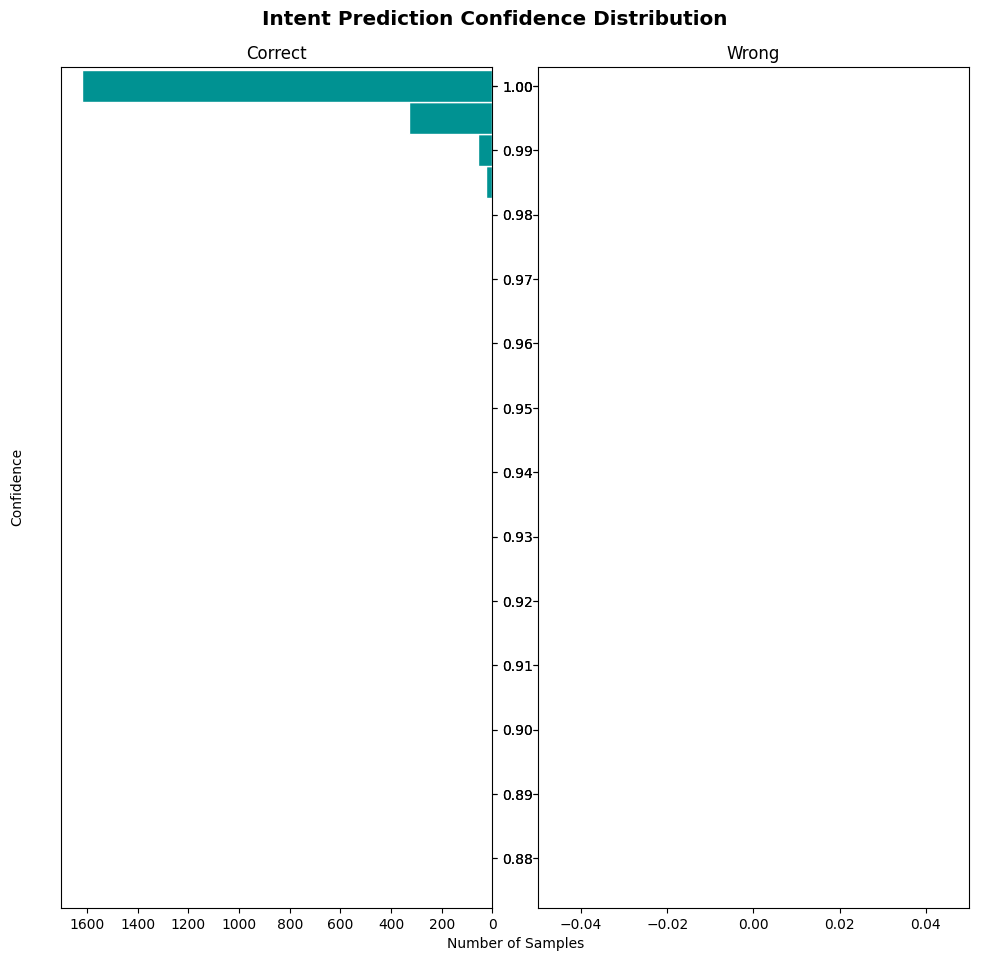
\includegraphics[angle=0,width=0.3\textwidth]{Figuras/intent_histogram.png}
	\caption{Histograma de confianza en la clasificación de Intenciones}
	\label{fig:intent_histograma}
\end{figure}
\subsubsection{Extracción de entidades}
Al ver los gráficos del extractor, tanto en la matriz de confusión de entidades
\ref{fig:entity_matriz} como en el histograma \ref{fig:entity_histograma} se encuentra que el
modelo se confunde con dos entidades, revisando el reporte de errores se encuentra que los
extractores DIETClassifier y EntitySynonymMapper reconocen las entidades por separado, esto genera
el error pero no afecta al rendimiento del modelo o a la correcta selección de una respuesta.

\begin{figure}[H]
	\centering
	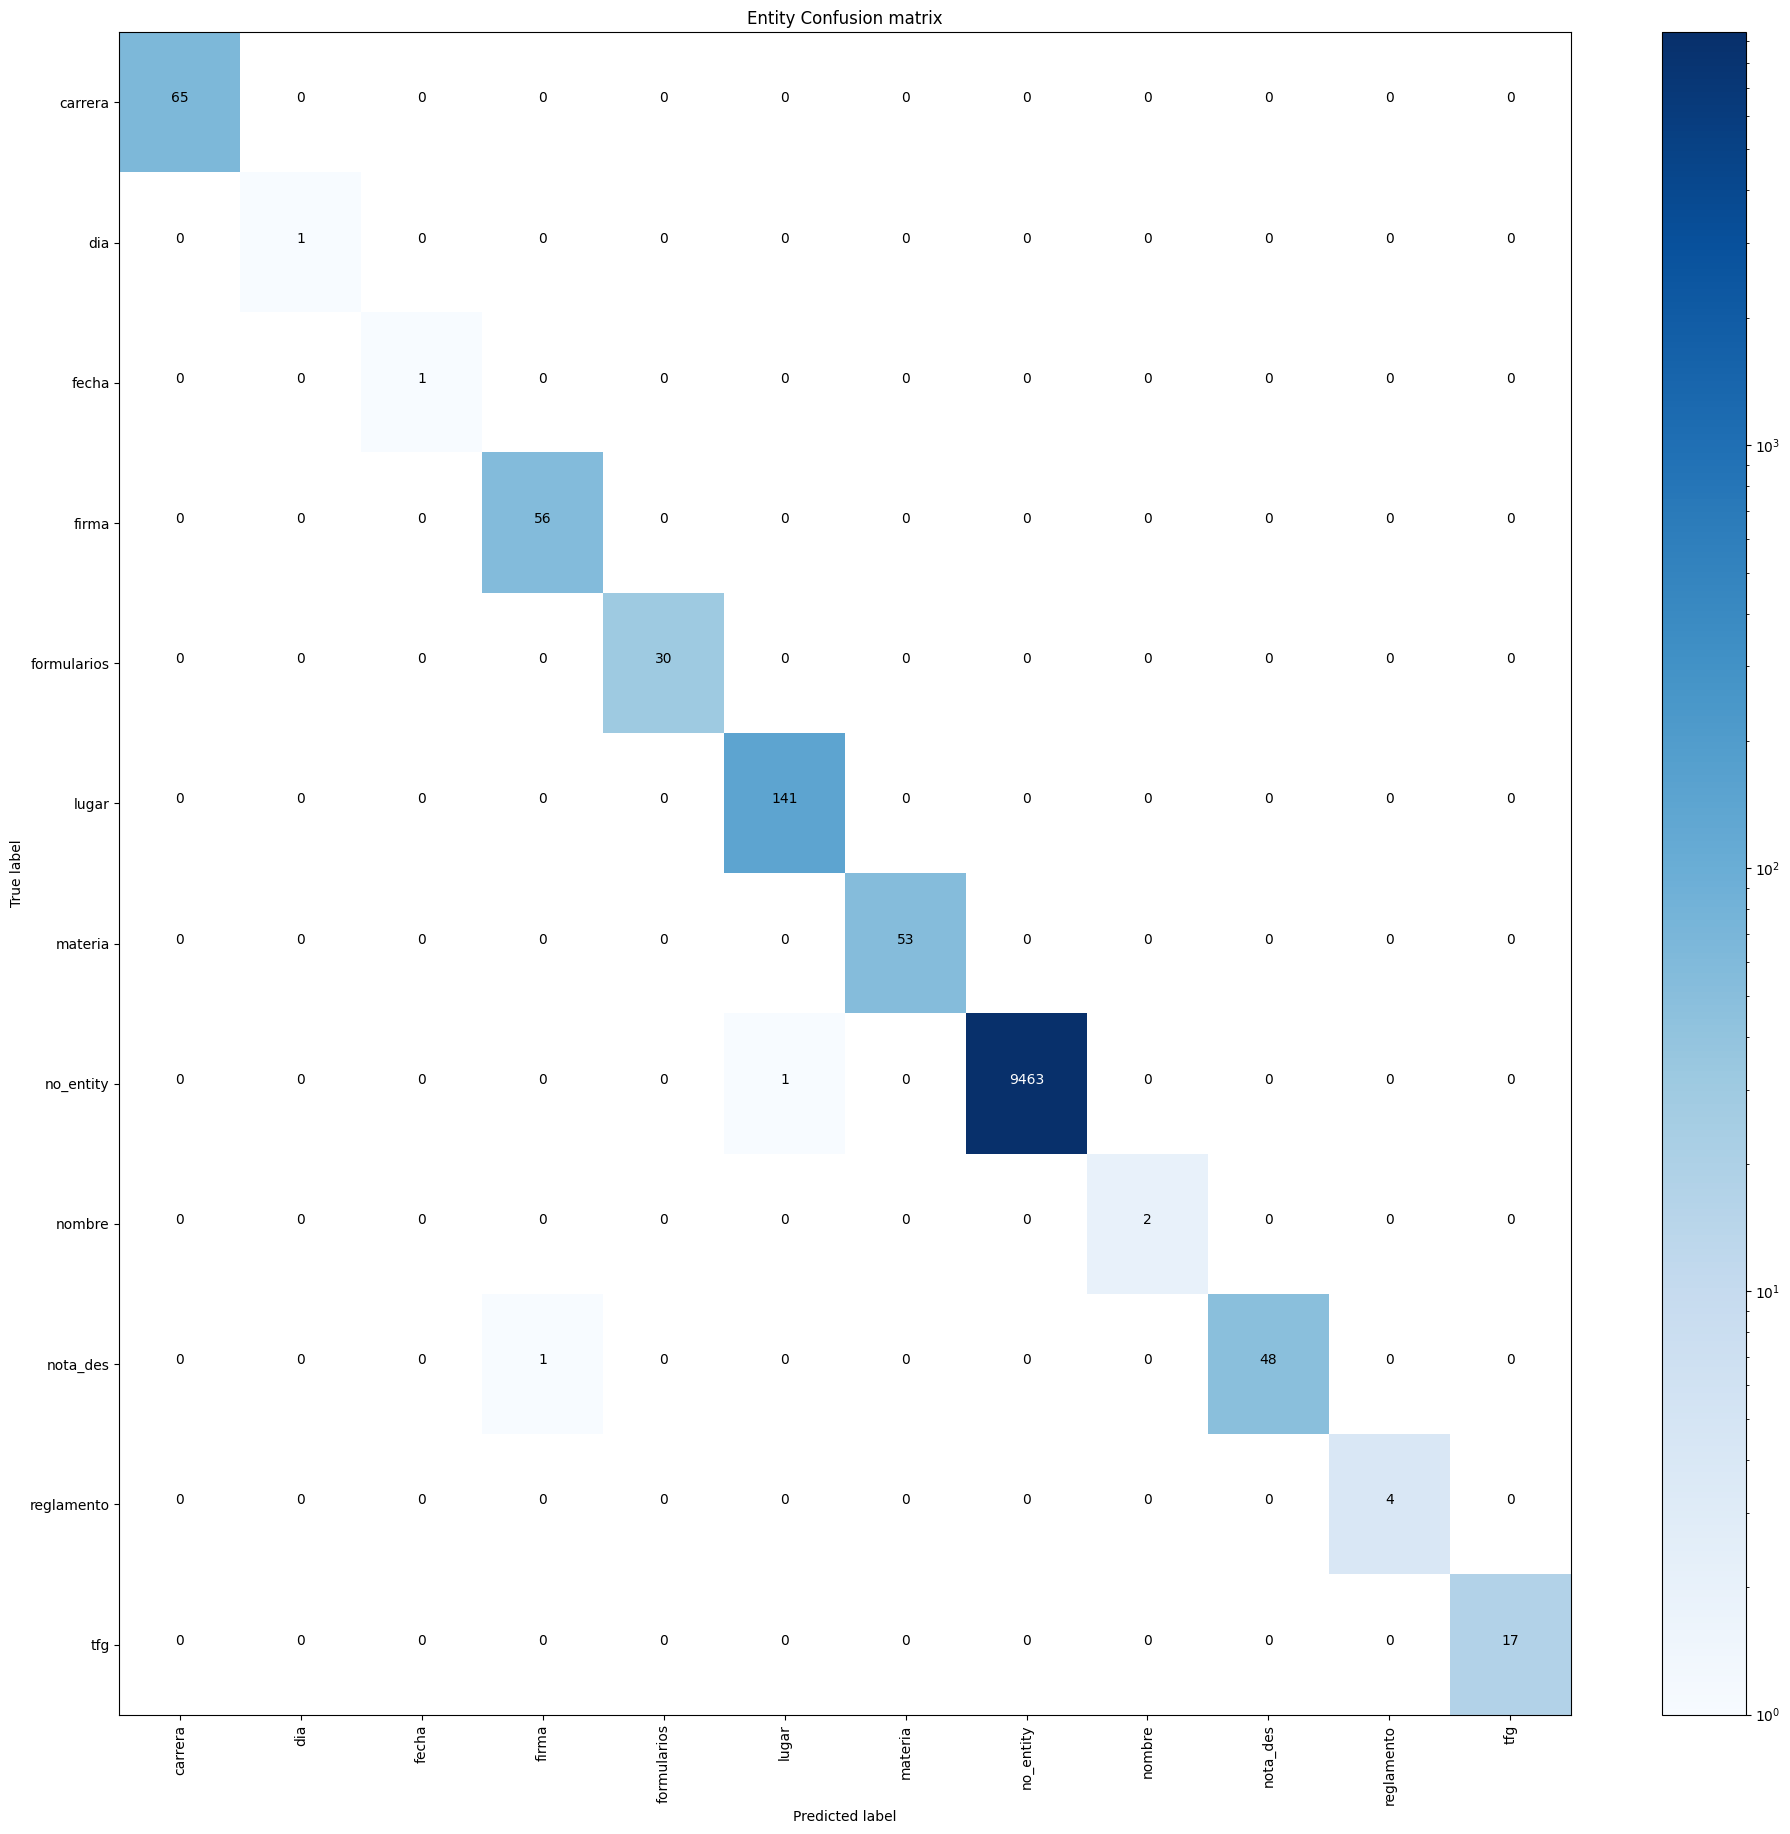
\includegraphics[angle=0,width=0.3\textwidth]{Figuras/DIETClassifier_confusion_matrix.png}
	\caption{Matriz de Confusión del extractor de entidades}
	\label{fig:entity_matriz}
\end{figure}

\begin{figure}[H]
	\centering
	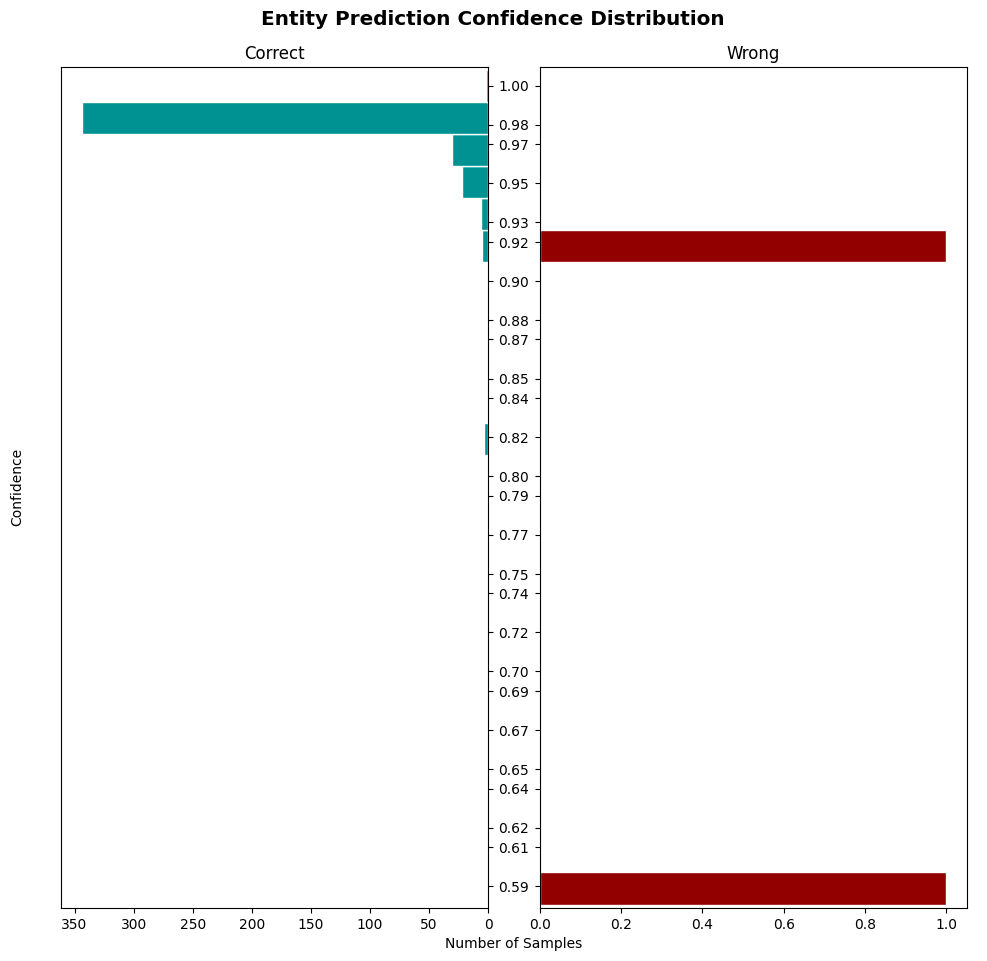
\includegraphics[angle=0,width=0.3\textwidth]{Figuras/DIETClassifier_histogram.png}
	\caption{Histograma de confianza del extractor de entidades}
	\label{fig:entity_histograma}
\end{figure}

\subsubsection{Selección de Respuestas}
Podemos observar en el histograma \ref{fig:response_histograma} de la selección de respuestas que
no se predijo erróneamente ninguna respuesta, la matriz de confusión en este caso no es de mucha
utilidad ya que son bastantes respuestas y complica la visibilidad de las etiquetas, en caso de que
existiese un error podremos encontrarlo en el reporte .json.

\begin{figure}[H]
	\centering
	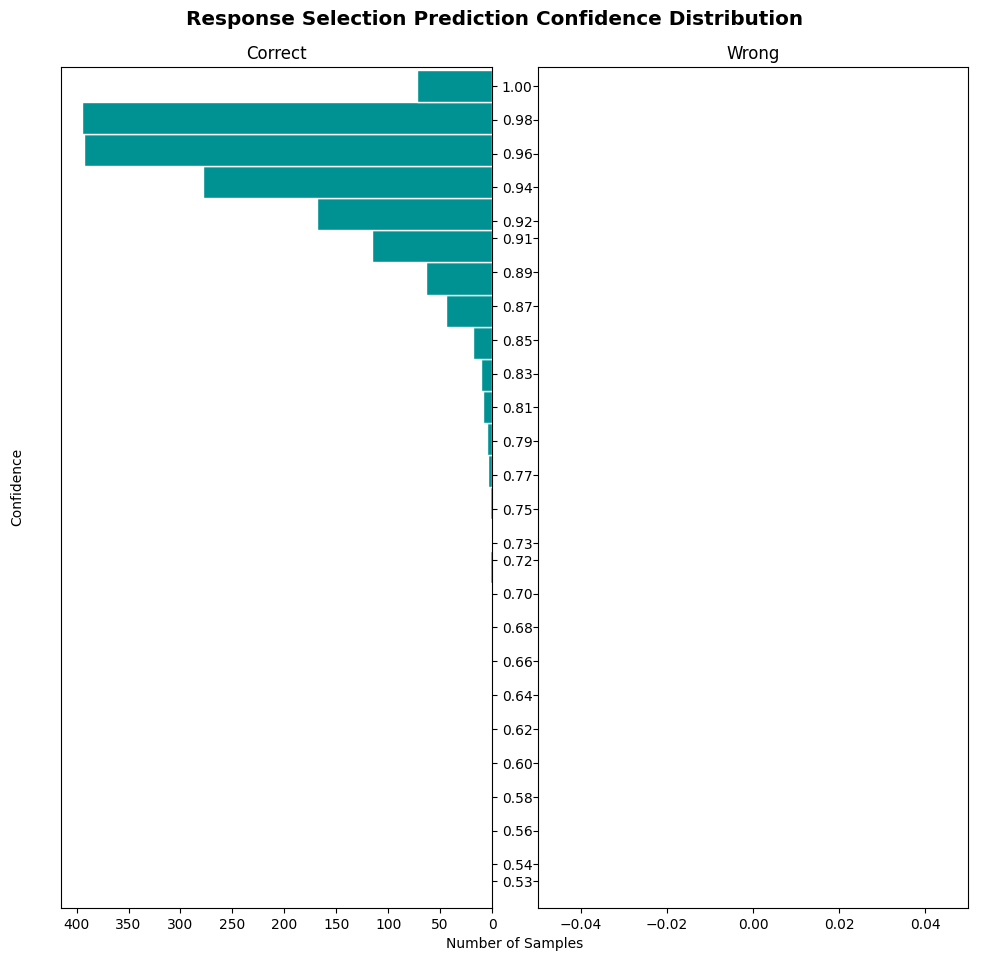
\includegraphics[angle=0,width=0.3\textwidth]{Figuras/response_selection_histogram.png}
	\caption{Histograma de confianza del seleccionador de respuestas}
	\label{fig:response_histograma}
\end{figure}
\section{Posibles Mejoras}
\begin{itemize}
	\item Integrar a sistemas existentes de la Facultad de Ingeniería.
	\item Autenticar usuarios a los sistemas de la Facultad de Ingeniería para obtener datos
	      específicos.
	\item Implementación de interfaz propia o utilización de elementos interactivos como
	      botones
	      para respuestas rápidas.
	\item Se puede agregar respuestas de la chatbots públicos como	ChatGPT \cite{api_chatgpt}
	      para preguntas
	      fuera del
	      contexto de la Facultad de Ingeniería.
\end{itemize}
